\documentclass[10pt]{article}\usepackage[]{graphicx}\usepackage[]{color}
%% maxwidth is the original width if it is less than linewidth
%% otherwise use linewidth (to make sure the graphics do not exceed the margin)
\makeatletter
\def\maxwidth{ %
  \ifdim\Gin@nat@width>\linewidth
    \linewidth
  \else
    \Gin@nat@width
  \fi
}
\makeatother

\usepackage{Sweavel}


\usepackage{hyperref}
\usepackage{url}
\usepackage[a4paper]{geometry}
\usepackage{a4wide}
\usepackage{float}
\usepackage[english]{babel}
\usepackage[utf8]{inputenc}
\usepackage{csquotes}
\usepackage{amsmath}
\usepackage{amssymb}
\usepackage{xspace}
\usepackage[numbers]{natbib}
\bibliographystyle{unsrtnat}
\usepackage{subcaption}
\usepackage[font={small}]{caption}
\usepackage{booktabs}
\usepackage{listings}
\usepackage{cleveref}
\usepackage{lipsum}
\newcommand{\approxtext}[1]{\ensuremath{\stackrel{\text{#1}}{=}}}
\newcommand{\matr}[1]{\mathbf{#1}}
\newcommand{\partt}[2]{\ensuremath{\dfrac{\partial {#1}}{\partial {#2}}}}
\renewcommand{\d}[1]{\ensuremath{\operatorname{d}\!{#1}}} % non-italized differentials
\newcommand{\h}[0]{\ensuremath{\hbar}} % hbar
\def\changemargin#1#2{\list{}{\rightmargin#2\leftmargin#1}\item[]}
\let\endchangemargin=\endlist 
\usepackage{amsthm}
\theoremstyle{plain}
\renewcommand{\theequation}{\thesection.\arabic{equation}}
\def\changemargin#1#2{\list{}{\rightmargin#2\leftmargin#1}\item[]}
\let\endchangemargin=\endlist    
\usepackage{xcolor}
\definecolor{Red}{rgb}{0.7,0,0}
\definecolor{Blue}{rgb}{0,0,0.8}
\usepackage{verbatim}
\def\changemargin#1#2{\list{}{\rightmargin#2\leftmargin#1}\item[]}
\let\endchangemargin=\endlist
\addtolength{\oddsidemargin}{-.35in}
\addtolength{\evensidemargin}{-.35in}
\addtolength{\textwidth}{.7in}
\usepackage{multicol}

% Stephen's stuff
\newcommand{\R}{\texttt{R}}
\newcommand{\Rfunction}[1]{{\texttt{#1}}}
\newcommand{\Robject}[1]{{\texttt{#1}}}
\newcommand{\Rpackage}[1]{{\mbox{\normalfont\textsf{#1}}}}
\usepackage{xcolor}
\definecolor{Red}{rgb}{0.7,0,0}
\definecolor{Blue}{rgb}{0,0,0.8}
\hypersetup{%
pdfusetitle,
bookmarks = {true},
bookmarksnumbered = {true},
bookmarksopen = {true},
bookmarksopenlevel = 2,
unicode = {true},
breaklinks = {false},
hyperindex = {true},
colorlinks = {true},
linktocpage = {true},
plainpages = {false},
linkcolor = {Blue},
citecolor = {Blue},
urlcolor = {Red},
pdfstartview = {Fit},
pdfpagemode = {UseOutlines},
pdfview = {XYZ null null null}
}
%% Listings
\lstset{ 
language=R,                     % the language of the code
basicstyle=\footnotesize,       % the size of the fonts that are used for the code
numbers=left,                   % where to put the line-numbers
numberstyle=\tiny\color{gray},  % the style that is used for the line-numbers
stepnumber=1,                   % the step between two line-numbers. If it's 1, each line will be numbered
numbersep=5pt,                  % how far the line-numbers are from the code
backgroundcolor=\color{white},  % choose the background color. You must add \usepackage{color}
showspaces=false,               % show spaces adding particular underscores
showstringspaces=false,         % underline spaces within strings
showtabs=false,                 % show tabs within strings adding particular underscores
rulecolor=\color{black},        % if not set, the frame-color may be changed on line-breaks within not-black text (e.g. commens (green here))
tabsize=2,                      % sets default tabsize to 2 spaces
captionpos=b,                   % sets the caption-position to bottom
breaklines=true,                % sets automatic line breaking
breakatwhitespace=false,        % sets if automatic breaks should only happen at whitespace
title=\lstname,                 % show the filename of files included with \lstinputlisting;
% also try caption instead of title
keywordstyle=\color{Blue},      % keyword style
commentstyle=\color{orange},    % comment style
stringstyle=\color{Red},        % string literal style
morekeywords={*,...}            % if you want to add more keywords to the set
} 


%%% Document specific
\newcommand{\course}{Population Genetics}
\newcommand{\ass}{1}
\newcommand{\term}{Lent term 2017}
%\bibliography{pga1}

%%% Title page
\title{
  \bf \course: Assignment \ass \\[1em]
  \small{University of Cambridge}
}

\author{Henrik Åhl}
\date{\today}
\renewcommand{\textfraction}{0.05}
\renewcommand{\topfraction}{0.8}
\renewcommand{\bottomfraction}{0.8}
\renewcommand{\floatpagefraction}{0.75}

%%% Actual document
\begin{document}
\date{\today}
\maketitle
\setcounter{page}{1}


% \date{\today}
\maketitle
% \begin{abstract}
% {\bf 
%   %\begin{changemargin}{-.8cm}{-.8cm}
%   This is an abstract abstract.
% }
% \end{abstract}

\begin{multicols*}{2}
\section*{Preface}
This is an assignment report in connection to the \textit{\course}
module in the Computational Biology course at the University of Cambridge,
\term. All related code is as of \date{\today} available through a
Github repository by contacting \href{mailto:hpa22@cam.ac.uk}{hpa22@cam.ac.uk}.

\section*{Exercises}
\subsection*{1 -- Measurement of variance}
\begin{enumerate}
  \item[A]~
    \begin{table}[H]
      \centering
      \vspace{-.6cm}
      \caption{Solution to exercise 1a}\label{tab:exc1}
      \begin{tabular}{c|ccc}
        \toprule
        &Selected  & $\neg$Selected  & Total [\%]\\
        \midrule
        $p^2$ &0.18  & 0.12  & 0.14 \\
        $2pq^2$ &0.49  & 0.45  & 0.47 \\
        $q^2$ &0.32  & 0.44  & 0.39 \\\bottomrule
      \end{tabular}
    \end{table}
  \item[B] The heterozygosity is the frequency of the middle row in~\cref{tab:exc1}.
  \item[C] We calculate $F_{ST} = 1 - \dfrac{2p_Sq_S}{2p_Tq_T} = 0.00836$. A low value in this would correspond to a situation where no
    difference in heterozygosity is prevalent between the subpopulations. In
    contrast, a high value would mean that the populations are completely
    segregated, with the respective alleles in each subpopulation being fixed. Indeed, this mirrors what we see in the statistics above. 
\end{enumerate}

\subsection*{2 -- Modelling fitness in a diploid system}
\begin{enumerate}
  \item[A] The Hardy-Weinberg proportions simply correpsond to the combinatorial
    probability of achieving a certain setup of alleles. Like before, it is
    thus simply $p^2$ for genotype $AA$, $2p(1-p)$ for $Aa$ and $aA$ (assuming they are equivalent), and $(1-p)^2$
    for aa. 
  \item[B] 
    
  The mean fitness is given by evaluating the different fractions which are
affiliated with a certain fitness. Retaining the algebraic form of our fitness
values before calculating, we get the following expression and subsequent result:
    \begin{align*}
      \bar f =&~(0.9a + 0.1)p^2 + 2(0.9b + 0.1)p(1-p) \\&+ c(1-p)
      ^2 = \\
      =&~0.84
    \end{align*}  


  \item[C] 
    Reducing our expression above further, we can choose to
    differentiate with respect to the probability. There is only extremum, which
    is a maximum, since the second derivative evaluates to $<0$.
    \begin{align*}
      \bar f &= 0.82p^2 + 1.82p(1-p) +
      0.7(1-p)^2 \\
      \dfrac{d\bar f}{dp} &= 1.64p + 1.82(1-2p) -
      1.4(1-p) \stackrel{!}{=} 0 \\
      p^* &= 0.7 \\
      \bar f_{p^*} &= 0.85
    \end{align*}
  \item[D] We transform our problem accordingly:
  \begin{table}[H]
     \centering
     \caption{Solution to exercise 2d}\label{tab:exc2d}
     \begin{tabular}{ccc}
       \toprule
       Genotype & Required form & Transformed form\\
       \midrule
     AA & $1 + 2\sigma$   & $1.17$ \\
     Aa & $1 + 2h\sigma$  & $1.29b + 0.14$ \\
     aa & $1$             & $1$ \\\bottomrule
     \end{tabular}
   \end{table}
   With our transformed values, solving for the unknowns gives us $\sigma = 0.086$ and $h = 7.5b - 5$. We can thereafter investigate for which values in our equation governing the rate of change is negative, which we require for fixation in the $q_A$ underdominance case. Relabelling $q$ as p, we get r.o.c.\ is given by 
   \begin{align*}
    \dfrac{dq}{dt} = 2\sigma p(1-p)(p + h(1-2p))
   \end{align*}
   where $p \in \left[0, 1\right]$. Only the last factor will therefore affect the sign of the derivative. Inserting our values reduces the informative part to
   \begin{align*}
      p + (7.5b - 5)(1 - 2p) \stackrel{!}{\leq} 0 
   \end{align*}
   where we now want to find the values fulfilling this. Solving for our parameters gives us that this occurs in the two regions    
   \begin{gather*}
      % b \in [\dfrac{2}{3}, 0.8] \\
      % b = \dfrac{11}{ 15} \\
      b > \dfrac{11}{15},\ p \geq \dfrac{5(3b-2)}{2(15b-11)} \\
      b < \dfrac{11}{15},\ p \leq \dfrac{5(3b-2)}{2(15b-11)}.
   \end{gather*}
   However, we are only interested in the over- and underdominance cases for $q_A$, i.e.\ for $h > 1$ and $h < 0$ respectively. Only in the latter case are we required to know the sign of the derivative. Our equation of $h = 7.5b - 5$, we therefore get that we have fixation of $q_a$ when $b > 0.8$ and $b < \dfrac{11}{15},\ p \leq \dfrac{5(3b-2)}{2(15b-11)}$, where the first corresponds to overdominance for $q_A$, and the latter underdominance.  

\end{enumerate}

\begin{Schunk}
\begin{figure}[H]

{\centering 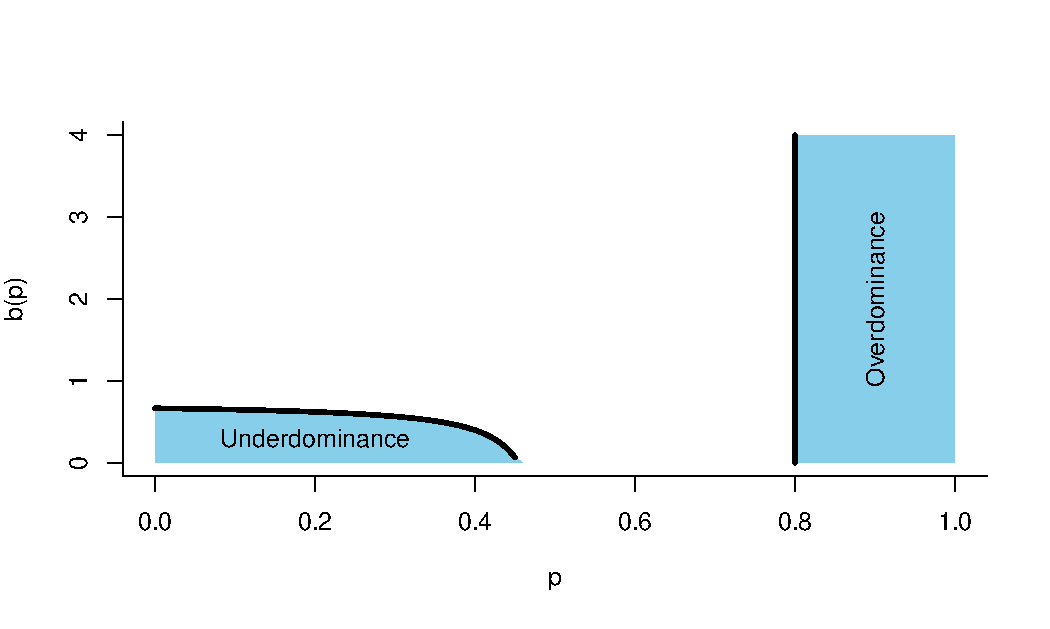
\includegraphics[width=\maxwidth]{figure/twocolumn-3_fixation-1} 

}

\caption[Fixation diagram for the allele $q_a$]{Fixation diagram for the allele $q_a$. The allele will fixate for values within the shaded areas, where under-/overdominance is given for $q_A$.}\label{fig:3_fixation}
\end{figure}
\end{Schunk}


\subsection*{3 -- Dynamics of allele frequency change}
\begin{Schunk}
\begin{figure}[H]

{\centering 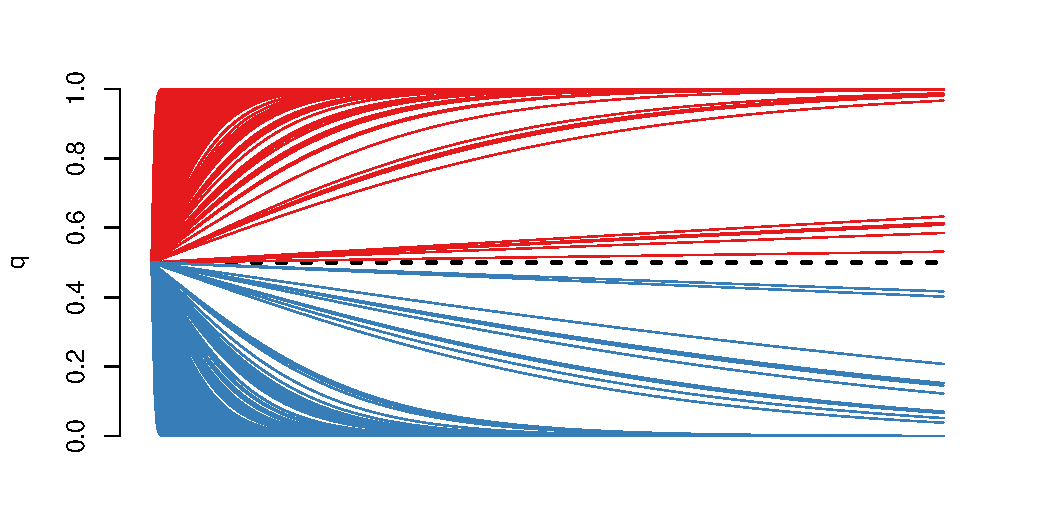
\includegraphics[width=\maxwidth]{figure/twocolumn-3_selection-1} 

}

\caption[Evolution trajectories for different values of the selection rate $\sigma$, with the popualation initalised at $q = 0.5$]{Evolution trajectories for different values of the selection rate $\sigma$, with the popualation initalised at $q = 0.5$. Naturally, negative values induce a negative pressure towards the allele, and it is as a consequence eradicated. Similarly, positive selection fixates the allele.}\label{fig:3_selection}
\end{figure}
\end{Schunk}
\begin{enumerate}
  \item[A] $\mu, \sigma$ and $N$ denote the mutation rate, the selection
    rate for a given allele, and the population size.
  \item[B] Under selective pressure, the allele is bound to either fixate or to
    simply die out. Whichever effect happens depends on the sign of $\sigma$,
    i.e.\ for $\sigma > 0$, the allele will eventually fixate with $q^1_i = 1$.
    In the contrasting case, the other allele will do the same. We can see this
    in \cref{fig:3_selection}, where we have separated randomly drawn positive values of $\sigma$ above in red, and correspondingly all negative values in blue.
  \item[C] With no selective pressure, and mutations frequently producing either allele, as well as under no genetic drift, we will get the effect outlined in \cref{fig:stochc}, namely that the population will trend towards an equilibrium with an even split between the fractions. How fast this effect happens depends inherently on the mutation rate, which is signified in the figure by colour.
\end{enumerate}
\begin{Schunk}
\begin{figure}[H]

{\centering 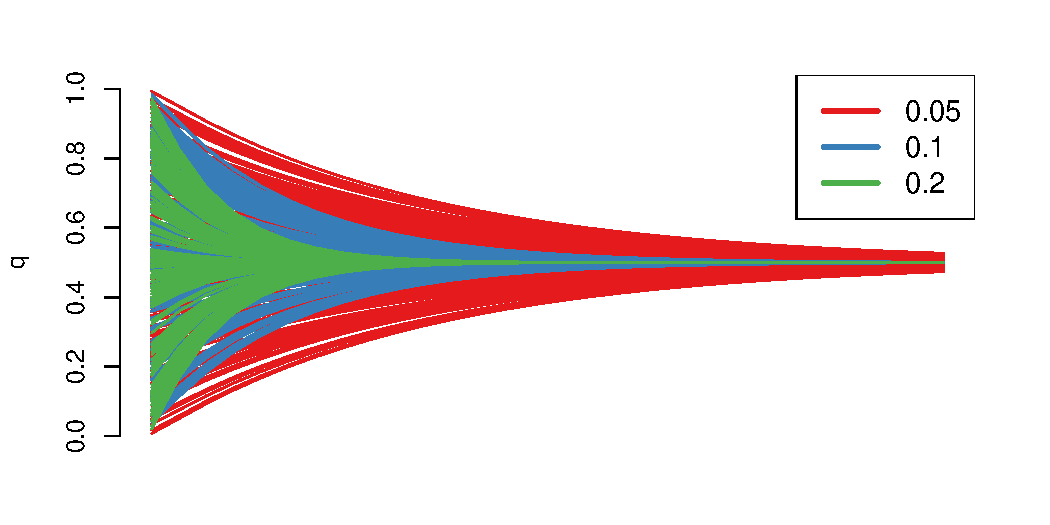
\includegraphics[width=\maxwidth]{figure/twocolumn-stochc-1} 

}

\caption[Population dynamics without any selective pressure]{Population dynamics without any selective pressure. The mutations will instead force the population to its stable equilibrium, with the rate of convergence depending on the mutation rate.}\label{fig:stochc}
\end{figure}
\end{Schunk}
\begin{enumerate}
  \item[D] \Cref{fig:stochd} shows 500 drift-driven simulations initialised at $q = 0.2$, as simulated under Stratonovich integration (using Milstein's method). As we can see, the population of simulations on the large spreads out uniformly due to no pressure in going towards either end. We can argue about how likely it is on the grand scale that a single simulation will reach an allele fraction of $q = 1$ by considering Kimura's equation first. Since the overall expression reduces to $\dfrac{\partial p}{\partial t} = 0$ for $x = 1$, the probability for all initial conditions is some constant over time, which must depend on the initial condition. Reducing the problem to a case of fewer individuals, it is easy to see that the probability of the allele fixating is equal to the initial frequency under no selective pressure. This is also what we see when we simulate our stochastic system sufficiently many times (data not shown, although hinted at in \cref{fig:stochd}). Another way to consider the problem is to imagine a setting where we have $N$ different alleles all with equal probability of fixating. At some point, on of them will have done so. Under no drift, the distribution of alleles for every generation can be traced back to the previous one, where the inheritance will depend directly on the prevalence of it. Reducing this all back to the origion, it is clear that the initial distribution will be equal to the probability of fixation.
\end{enumerate}
\begin{Schunk}
\begin{figure}[H]

{\centering 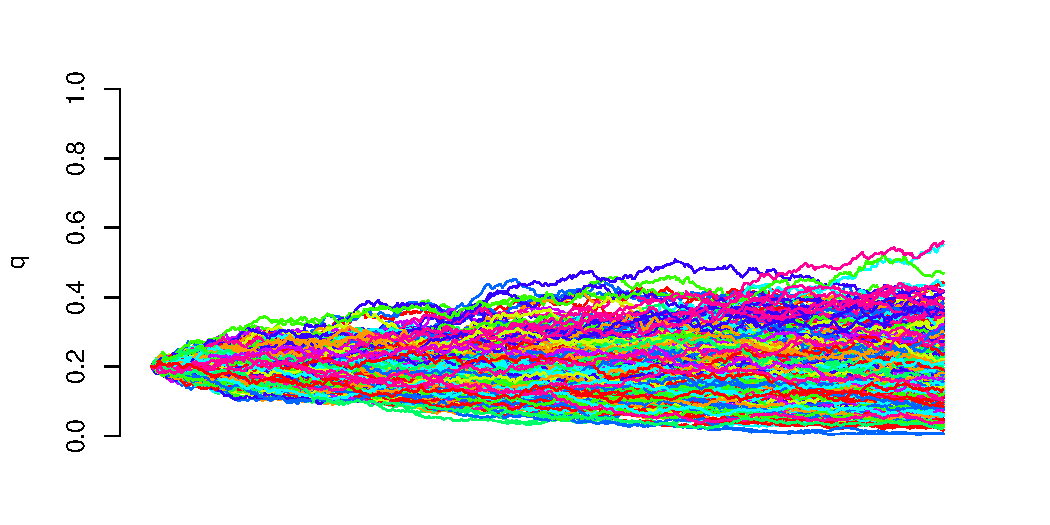
\includegraphics[width=\maxwidth]{figure/twocolumn-stochd-1} 

}

\caption[Curves for 500 drift-driven simulations]{Curves for 500 drift-driven simulations. Note how the population spreads out uniformly around its initial condition.}\label{fig:stochd}
\end{figure}
\end{Schunk}

\subsection*{4 -- Time-dependent selection}
\begin{enumerate}
  \item[A] We separate our expression into two parts, and use induction to reason our way to the final answer. In particular, we have 
  \begin{align*}
  x(t')   =&~\dfrac{x_0e^{\sigma_1t'}}{1 - x_0 + x_0 e^{\sigma_1t'}} \\
  x(t>t') =&~\dfrac{x_{t'}e^{\sigma_2(t-t')}}{1 -  x_{t'} + x_{t'}e^{\sigma_2(t-t')}} = \\
          =&~\dfrac{x_0 e^{\sigma_2(t-t') + \sigma_1t'}}{\left(1 - x_0 + x_0e^{\sigma_1t'}\right)} \times \\
         &\times \dfrac{1}{\left(1 - \dfrac{x_0e^{\sigma_1t'} + x_0e^{\sigma_1t' + \sigma_2(t-t')}}{
            1 - x_0 + x_0e^{\sigma_1t'}}\right)} = \\
          =&~\dfrac{x_0e^{\sigma_1t' + \sigma_2(t-t')}}{1 - x_0 + x_0e^{\sigma_1t' + \sigma_2(t-t')}}
  \end{align*}
  for some arbitrary intervals where our $\sigma$'s are separable. Since we can repeat this process for any number of intervals, our corresponding exponent will equal a sum over the $\sigma_i\cdot t_i$ products, which in the limit of our timesteps trending towards zero is equivalent to our sought-after Riemann sum, i.e.\ integral, over the range.
  \end{enumerate}

\begin{enumerate}
  \item[B] It is not clear whether the variable $x$ corresponds to the allele frequency, or if it simply serves as an abstract, continuous genotype representation. Nevertheless, we choose to impose bounds such that the variable is restricted within the range $[0, 1]$. 
  
  As we can see in \cref{fig:fisherb}, the population of smaller size is affiliated with a much larger variability, as is to be expected from the expression defining the probability of a fixation. In contrast, the larger population steadily reaches the optimum and does not sway further on. As given in the formula, the larger population size simply keeps the probability of fixation down. Far away from the optimum, the regression in fitness caused by a non-beneficial fixation is not relatively as bad, which is why we some some variance in the beginning. 
  
  Because of the rigid optimum, the accumulated fitness variations mirror precisely the fraction trajectory. Because the optimum is static, we see a direct mirroring in the change in fitness from the change in $x$. 
\end{enumerate}

\begin{Schunk}
\begin{figure}[H]

{\centering 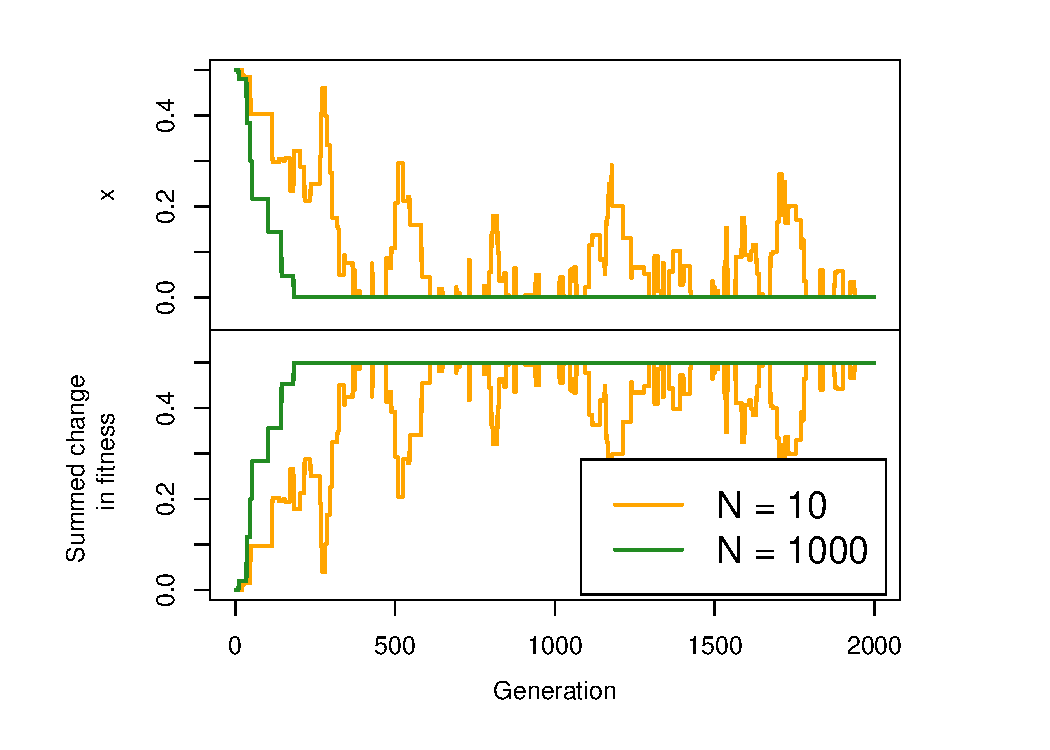
\includegraphics[width=\maxwidth]{figure/twocolumn-fisherb-1} 

}

\caption[Change in $x$]{Change in $x$}\label{fig:fisherb}
\end{figure}
\end{Schunk}
\begin{enumerate}
  \item[C] Inducing oscillations, we see very different dynamics in the system than before. \Cref{fig:fisherc} shows how the two populations try to adapt to the changing fitness. As the accumulated fitness change shows, the larger population has a higher trend-curve, which again shows the signs of lesser variance. Since the smaller population more oftenly fixates in the 'wrong' direction, the cumulative trend will be sligthly lower, as we observe. We also note how both populations are able to adapt decently, although the larger population does so in a more stable manner.  
\end{enumerate}

\begin{Schunk}
\begin{figure}[H]

{\centering 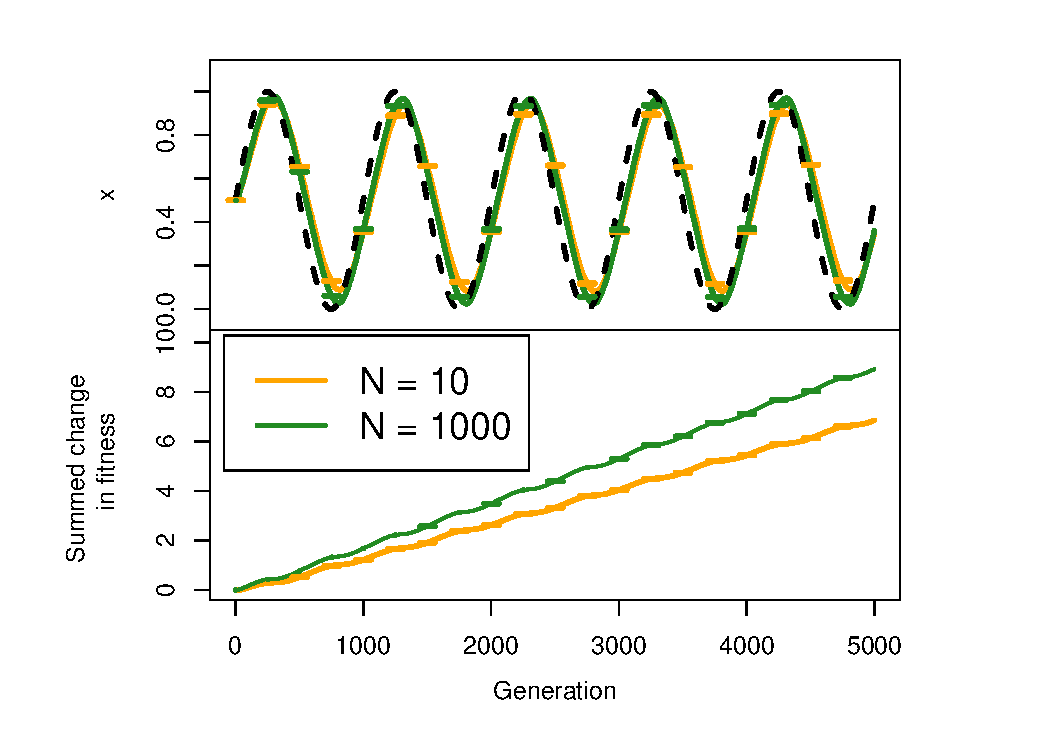
\includegraphics[width=\maxwidth]{figure/twocolumn-fisherc-1} 

}

\caption{Dynamics for the same scenario as \cref{fig:fisherb}, but with a sinusoidally changing optimum around 0.5. Note how both populations are able to adapt to the changing fitness, but with different local variance.}\label{fig:fisherc}
\end{figure}
\end{Schunk}
\begin{enumerate}
  \item[D] \Cref{fig:fisherd,fig:fisherd_ext} show thr dynamics when the rate of the oscillations increase, with exemplary curves and the mean over 100 simulations respectively. Like in the previous case, the smaller population is affiliated with larger fluctuations, which shows similarly to previously in the cumulative change (\cref{fig:fisherd_ext}). Nevertheless, both populations are generally able to adapt to the fluctuations, although the smaller population size still has a higher tendency to shift in the wrong direction. As the mean trend in particular shows, however, the increase in oscillatory rate pushes the populations towards the mean of the fitness value. The rapid change of the optimum is simply too much for the populations in order for them to adapt in time, which becomes the more apparent the higher the oscillations. Still, we again see the general trend in the larger population size being able to follow the optimum better in general. Even though the smaller population size in theory allows it to "jump past" the optimum, it does not prove a sufficiently competetive trait in this setting.
  
  However, a system under varying oscillatory rate will never completely pan out and average to the center, as this depends on the phase of the curve. In some cases the two will be in phase in such a way that the $x$ variable is driven towards the ends. This nevertheless depends inherently on the development of $\lambda$, and other oscillating systems might circumvent this. Still, we see the a \textit{trend} towards the mean of the oscillations, which is indeed telling of the overall dynamics. In a biological system, we would likely see that same general trend, with a bias towards staying close to the average, given that we would have a fitness landscape which depends on one variable. In reality, this is of course rarely the case, and movement on the fitness landscape happens in much more complex ways, through means of for example neutral mutations, which are unaccounted for here. We can nevertheless still infer that there would be a pressure towards \textit{adaptability}, which would prevent the population from reaching its optimum, and instead making it transverse intermediate state that allow for rapidly climbing towards new optima. 
  
  Bacteria cultures could be an example of a population type which have assumed this fast-paced adaptive approach, with large population numbers being able to react to rapid changes in the environment (and hence fitness landscape). In contrast, a smaller population size would make the system a lot more susceptible to changes in the environment, which might prove useful in some cases, but also detrimental to the population as a whole. 
\end{enumerate}

\begin{Schunk}
\begin{figure}[H]

{\centering 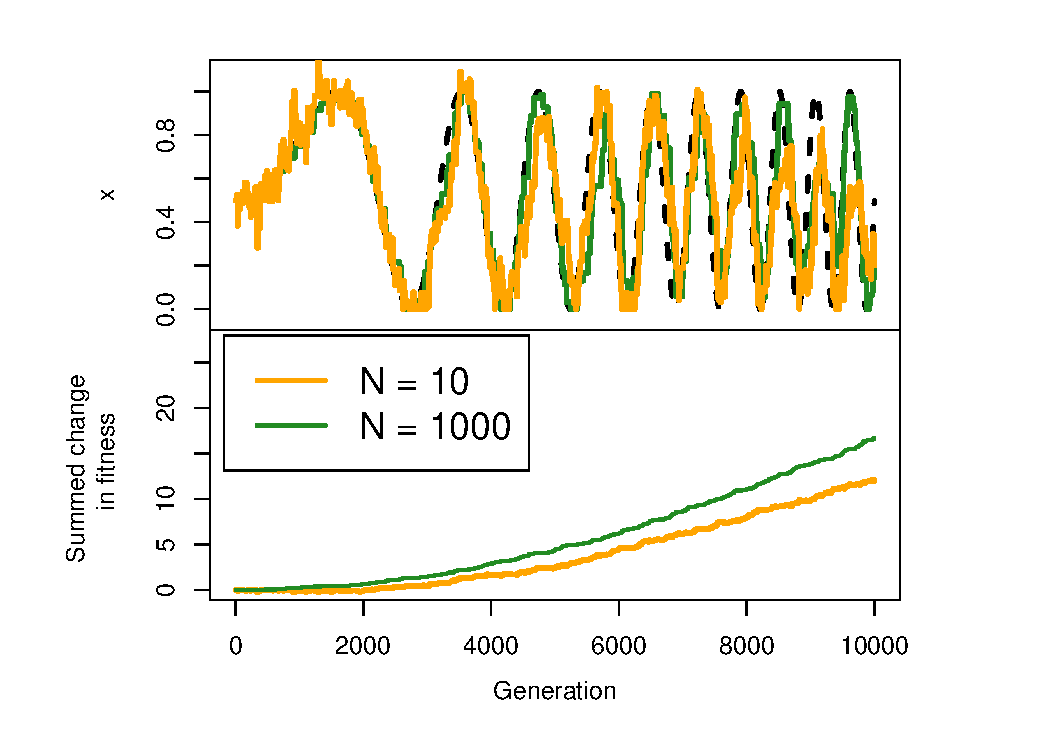
\includegraphics[width=\maxwidth]{figure/twocolumn-fisherd-1} 

}

\caption[$\lambda$ ranging linearly between 0.001 and 0 over the 10000 generations]{$\lambda$ ranging linearly between 0.001 and 0 over the 10000 generations.}\label{fig:fisherd}
\end{figure}
\end{Schunk}

\begin{Schunk}
\begin{figure}[H]

{\centering 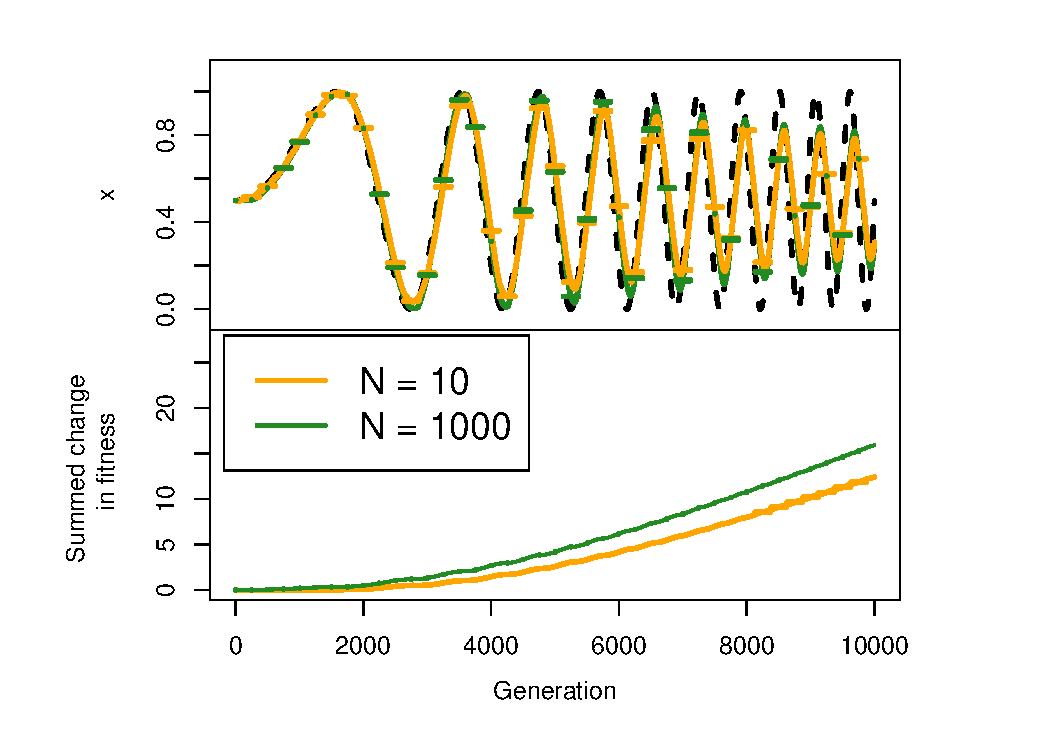
\includegraphics[width=\maxwidth]{figure/twocolumn-fisherd_ext-1} 

}

\caption{Mean and standard error for 1000 simulations in the same setting as in \cref{fig:fisherd}. Note how a slight trend in the adaptability is apparent, with the smaller population consistently being less able to reach an adequate fitness.}\label{fig:fisherd_ext}
\end{figure}
\end{Schunk}

\bibliography{references}
\end{multicols*}
\newpage
\onecolumn
  \appendix
\section{Code}
   \lstinputlisting{../code/stoch.R}
   \lstinputlisting{../code/stochc.R}
   \lstinputlisting{../code/stochd.R}
   \lstinputlisting{../code/fisherb.R}
   \lstinputlisting{../code/fisherc.R}
   \lstinputlisting{../code/fisherd.R}
   \lstinputlisting{../code/fisherd_ext.R}
\end{document}
